\documentclass[12pt,a4paper]{article}

\usepackage[utf8]{inputenc}
\usepackage[greek,english]{babel}
\usepackage{float}
\usepackage[export]{adjustbox}
\usepackage{sans} 
\usepackage{kerkis} 
%\usepackage{sans}
%\usepackage[LGRgreek]{mathastext}   
\usepackage{graphicx}
\usepackage{enumerate}
%\usepackage{enumitem}  
\usepackage{amsmath}
\usepackage{hyperref,xcolor} 
\usepackage{subcaption}

\hypersetup{
    colorlinks,
    linkcolor={black!50!black},
    citecolor={blue!50!black}, urlcolor={cyan!80!black},
}

\newcommand{\en}{\selectlanguage{english}} 
\newcommand{\tl}{\textlatin} 
\newcommand{\gr}{\selectlanguage{greek}}   
\newcommand{\code}[1]{\texttt{#1}}         
%\newcommand{\tsuper}{\textsuperscript} \newcommand{\tsub}{\textsubscript}

 %\renewcommand{\thesection}{\arabic{section}.} 
% \renewcommand{\thesubsection}{\arabic{subsection}.}


\gr \title{{\bf 
\includegraphics[scale=1.0]{images/up_landscape.jpeg} \\ ΤΜΗΜΑ ΜΗΧΑΝΙΚΩΝ ΗΛΕΚΤΡΟΝΙΚΩΝ ΥΠΟΛΟΓΙΣΤΩΝ ΚΑΙ ΠΛΡΟΦΟΡΙΚΗΣ  \\ \vspace{3cm}Αναφορά Εργαστηριακής Άσκησης Μέρος Β' \\ Υπολογιστική Νοημοσύνη}}
\author{Κωνσταντίνος Τσάκωνας \\ Α.Μ.: 1059666}
\date{Ακαδημαϊκό έτος 2020-21\\ Εαρινό Εξάμηνο}

\begin{document}

    \gr \maketitle \newpage

%    \tableofcontents  \newpage

    \section*{\tl{Repository} \gr Κώδικα}
        Για την ανάπτυξη της άσκσης χρησιμοποιήθηκε η γλώσσα \tl{Python} με τις βιβλιοθήκες \tl{Tensorflow, numpy, pandas, deap} και \tl{matplotlib}. Παρακάτω υπάρχει το \tl{repository} του κώδικα στο \tl{github} \\
        \underline{\tl{\textbf{\href{https://github.com/iamtsac/computational-intelligence-part-b}{github link}}}}

        \section*{Β1. Σχεδιασμός ΓΑ}
            \begin{enumerate}[a)]
                \item Τα άτομα του αρχικού πληθυσμού θα αναπαραστηθούν ως
                    δυαδικές συμβολοσειρές. Ο λόγος που θα ακολουθηθεί αυτή η
                    κωδικοποίηση προέρχεται από το σκεπτικό ότι, αυτό που
                    θέλουμε να κάνουμε είναι να μειώσουμε το εισόδους από τα 784
                    \tl{pixels}, δηλαδή να μηδενίσουμε πολλές από αυτές.
                    Δημιουργώντας λοιπόν άτομα του πληθυσμού ως πίνακες 784
                    \tl{pixels} που περιέχουν δυαδικά στοιχεία, μπορούμε με ένα
                    πολλαπλασιασμό \tl{element-wise} να κρατήσουμε τις εισόδους που
                    θέλουμε.
                \item Ο αρχικός πληθυσμός θα είναι \tl{N} τυχαίοι πίνακες(τυχαία
                    δειγματοληψία)
                    28\tl{x}28 και οι τιμές που θα περιέχουν θα είναι 0 και 1.
                \item Η συνάρτηση καταλληλότητας που επιλέχθηκε είναι οι εξής:
                    \begin{itemize}
                        
                        \item κάθε φορά που θα γίνεται έλεγχος στο νευρωνικό
                            σύμφωνα με τις εισόδους που προκύπτουν από κάθε
                            άτομο του πληθυσμού θα κάνουμε ταξινόμηση των πρώτων
                            $10.000$ εικόνων και θα συγκρίνουμε την ταξινόμηση
                            αυτή με βάση τα \tl{labels} για να δούμε πόσο
                            ακριβής είναι. Το αποτέλεσμα ου θα προκύπτει από
                            αυτό θα είναι μια τιμή μεταξύ του διαστήματος
                            $[0,1]$
                            και στόχος του γενετικού αλγορίθμου θα είναι να
                            πλησιάσει όσο το δυνατό πιο κοντά στο $1$.
                        \item Επίσης θα επιβάλλεται μία ποινή σε άτομα του
                            πληθυσμού που έχουν μεγάλο αριθμό εισόδων,
                            συγκεκριμένα άτομα που έχουν περισσότερες από $300$
                            εισόδους. Η τιμή η οποία θα αφαιρείται είναι
                            ανάλογη με το σφάλμα της ταξινόμησης δια εκατό επί
                            το πλήθος των παραπάνω εισόδων που έχει σε σχέση με
                            αυτές που έχουμε θέσει ως επιθυμητό άνω όριο.
                            Δηλαδή:
                            $$ f(i) = acc_i - \frac{loss_i}{100}*(inputs_i - limit)$$

                    \end{itemize}
                    Ο λόγος που επιλέχθηκε η μεγιστοποίηση του ποσοστού
                    ταξινόμησης έχει να κάνει με το γεγονός ότι κατά την δημιουργία και την
                    εκπαίδευση του μοντέλου στην προηγούμενη εργαστηριακή άσκηση
                    σε πάρα πολύ μικρές τιμές του \tl{loss} η ταξινόμηση δεν
                    ήταν πάντα σωστή και δεν συμβάδιζε με το \tl{accuracy} του
                    μοντέλου. Ακόμα ο λόγος που εφαρμόζουμε ποινή σε άτομα που
                    έχουν περισσότερες από $300$ εισόδους είναι γιατί θα έχουμε
                    μία μείωση πάνω από $50\%$ αλλά για λιγότερες εισόδους από αυτές θα
                    χάνουμε χαρακτηριστικά που χρειαζόμαστε αφού το σχήμα των
                    ψηφίων στις εικόνες συνεχώς μεταβάλλεται, με αποτέλεσμα να
                    μην έχουμε καλή ταξινόμηση.

                \item Γενετικοί Τελεστές:
                    \begin{enumerate}[i.]
                        \item Επιλογή:
                        \begin{itemize}
                                \item Ρουλέτα βάσει κόστους: Με αυτή την μέθοδο από Ν 
                                    άτομα επιλέγουμε με βάση μία 
                                    πιθανότητα \tl{$p_i$} τα άτομα τα οποία θα γίνει η διασταύρωση. Η 
                                    πιθανότητα υπολογίζεται ως εξής: 
                                    $$ p_i = \frac{f_i}{\sum_{i=1}^{N}f_i}$$
                                     όπου, \\ $f_i$: το \tl{fitness} του \tl{i}-οστού ατόμου,\\
                                    Ν: το μέγεθος του πληθυσμού.
                                    \\ Κατά αυτό τον τρόπο τα άτομα με το μεγαλύτερο \tl{fitness} 
                                    έχουν μεγαλύτερη πιθανότητα να επιλεγούν, δηλαδή βαραίνουν περισσότερο.
                                    \item  Ρουλέτα βάσει κατάταξης: Με την μέθοδο αυτή τα 
                                        άτομα κατατάσσονται
                                        σύμφωνα με την καταλληλότητα σε αύξουσα σειρά. Στο 
                                        άτομα με τη μικρότερη 
                                        καταλληλότητα ανατίθεται κατάταξη 1, στο αμέσως επόμενο 2
                                        και η διαδικασία συνεχίζεται μέχρι το
                                        καταλληλότερο άτομα να έχει κατάταξη Ν, όπου 
                                        Ν το μέγεθος του πληθυσμού.
                                        Το μέγεθος που πιάνει το άτομο πάνω στη ρουλέτα σε 
                                        τοις εκατό προκύπτει από:
                                        $$\frac{r_i}{\sum_{i=1}^{N}r_i}\times100$$
                                        όπου,
                                        \\ $r_i$: η κατάταξη του \tl{i}-οστού ατόμου,\\ 
                                        Ν: το μέγεθος του πληθυσμού.
                                        \\ Σύμφωνα με το παραπάνω τα άτομα βαρύνουν με 
                                        τον ίδιο τρόπο ανεξαρτήτως της
                                        μεγάλης απόκλισης που μπορεί να έχει η συνάρτηση 
                                        καταλληλότητας τους.
                                        \\
                                    \item Τουρνουά: Με την μέθοδο αυτή 
                                        δημιουργούμε ένα τουρνουά μεγέθους Κ. Σε κάθε 
                                        τουρνουά διαλέγουμε τυχαία Κ άτομα, από αυτά επιλέγεται αυτό 
                                        με το καλύτερο 
                                        \tl{fitness}. %Τα άτομα που παιρνάνε στην
                                        %επόμενη γενιά δεν αφαιρούνται από τον πληθυσμό με αποτέλεσμα να μπορούν να 
                                        %επιλεγούν ξανά.
                                        \\
                        \end{itemize}
                        Από αυτές αυτή που επιλέχθηκε για τον αλγόριθμο μας σύμφωνα με το πρόβλημα 
                        που έχουμε να 
                            επιλύσουμε είναι η μέθοδος του Τουρνουά. Ο λόγος που επιλέχθηκε
                            βασίζεται στο γεγονός ότι
                            τα άτομα που θα επιλεγούν για να διασταυρωθούν θα έχουν μεγαλύτερες
                            διαφοροποιήσεις μεταξύ τους, διότι επιλέγονται Κ άτομα τυχαία. 
                            Στις υπόλοιπες μεθόδους 
                            οι επιλογή γίνεται με βάση κάποια πιθανότητα από τον αρχικό πληθυσμό με 
                            αποτέλεσμα τα άτομα
                            με καλύτερη καταλληλότητα να είναι πιο πιθανό να μην επιλεγούν. Άρα με την 
                            χρήση του τουρνουά και
                            την ποικιλομορφία που προσφέρει στη διασταύρωση μπορεί να προκύψει κάποιο 
                            άτομο με πολύ
                            καλύτερο \tl{fitness} από το καλύτερο άτομο της προηγούμενης γενιάς 
                            με αποτέλεσμα ο αλγόριθμος
                            να συγκλίνει πιο γρήγορα.
                    \item Διασταύρωση: 

                        \begin{itemize}
                                \item Διασταύρωση μονού σημείου: Κατά την
                                    διασταύρωση μονού σημείου δημιουργούνται
                                    ζευγάρια ατόμων από αυτά που επιλέχθηκαν και
                                    επιλέγεται τυχαία ένας ακέραιος αριθμός Ν.
                                    Τα άτομα είναι μήκους Μ και ισχύει ότι 
                                    $0\leqΝ\leqΜ-1$. Το Ν είναι το σημείο που θα
                                    γίνει η διασταύρωση των ατόμων, δηλαδή θα
                                    γίνει ανταλλαγή των δυαδικών ψηφίων Ν μέχρι
                                    $Μ-1$.
                                \item Διασταύρωση διπλού σημείου: Η μέθοδος
                                    είναι ίδια με την παραπάνω με την διαφορά
                                    ότι επιλέγονται δύο ακέραιοι αντί ενός και η
                                    διασταύρωση θα γίνει μεταξύ των δυαδικών
                                    ψηφίων που περιέχονται εντός των ορίων που
                                    θέτουν οι ακέραιοι που επιλέχθηκαν.
                                \item Ομοιόμορφη διασταύρωση: Για αυτού του
                                    τύπου την διασταύρωση δημιουργείται μια
                                    φόρμα από δυαδικά ψηφία μήκους ίδιου με του
                                    ατόμου. Στα σημεία που η φόρμα έχει τον
                                    ψηφίο 1 το πρώτο παιδί παίρνει το αντίστοιχο
                                    ψηφίο του δεύτερου γονέα, ενώ το δεύτερο παιδί του
                                    πρώτου γονέα. Όταν το ψηφίο της φόρμας είναι
                                    0 το πρώτο παιδί παίρνει το αντίστοιχο ψηφίο
                                    το πρώτου γονέα ενώ το δεύτερο παιδί του
                                    δεύτερου γονέα.\\
                        \end{itemize}
                         Στον αλγόριθμο μας επιλέξαμε διασταύρωση διπλού σημείο.
                         Εστιάζοντας στο πρόβλημα που έχουμε, πρέπει να
                         αφαιρέσουμε \tl{pixels} από μία εικόνα αλλά ταυτοχρόνως
                         να μην αφαιρέσουμε σημαντική πληροφορία για το
                         νευρωνικό μας. Οπότε με η διασταύρωση διπλού σημείου θα
                         μας προσφέρει μεγαλύτερη διαφοροποίηση στους απογόνους
                         από τους γονείς, πράγμα που επιζητούμε λόγω της
                         διαφορετικού τρόπου αναπαράστασης των αριθμών που
                         έχουμε να ταξινομήσουμε. Αν χρησιμοποιούσαμε ομοιόμορφη διασταύρωση θα είχαμε
                         πολλαπλά σημεία κοπής στους γονείς με αποτέλεσμα να
                         ανακατεύεται το γενετικό υλικό και να χάνουμε χρήσιμη
                         πληροφορία. Αν χρησιμοποιούσαμε διασταύρωση μονού
                         σημείου μετά από κάποιες γενεές οι απόγονοι θα μοιάζουν
                         πολύ με τους γονείς με αποτέλεσμα η καλύτερη λύση να
                         είναι κάποιο τοπικό ακρότατο.\\

                     \item  Μετάλλαξη: Η μετάλλαξη βοηθάει τον αλγόριθμό να
                         εξερευνήσει λύσεις σε όλο το επίπεδο λύσεων. Ο
                         ελιτισμός ουσιαστικά περνάει τα άτομα με το καλύτερο
                         \tl{fitness} αμετάλλακτα στην επόμενη γενιά. Επιλέξαμε
                         να ην χρησιμοποιήσουμε τον ελιτισμό διότι η μετάλλαξη
                         όπως είπαμε βοηθάει να γίνει εξερεύνηση περισσότερων
                         λύσεων και επίσης σε περίπτωση που έχουμε μικρό
                         πληθυσμό θα επωφεληθεί πολύ από αυτό. Σύμφωνα με το
                         δικό μας πρόβλημα επειδή χρησιμοποιούμε 10.000 εικόνες
                         από τις 60.000, ο ελιτισμός μπορεί να οδηγήσει σε
                         υπερπροσαρμογή την βέλτιστη λύση πάνω σε αυτές τις
                         10.000 εικόνες και να μειώσει την γενικευτική ικανότητα
                         του δικτύου.

                        
                    \end{enumerate}

            \end{enumerate}

            \section*{Β3. Αξιολόγηση και επίδραση παραμέτρων}
                \begin{enumerate}[a)]


                    \item Πίνακς αποτελεσμάτων \\
                     \begin{tabular}{|p{2em}| p{7em} | p{7em} | p{7em} | p{6.5em} | p{6em} | }
                        \hline
                        \textbf{Α/Α} & \textbf{ΜΕΓΕΘΟΣ ΠΛΗΘΥΣΜΟΥ} &
                        \textbf{ΠΙΘΑΝΟΤΗΤΑ
                            ΔΙΑΣΤΑΥΡΩΣΗΣ} & \textbf{ΠΙΘΑΝΟΤΗΤΑ
                        ΜΕΤΑΛΛΑΞΗΣ} & \textbf{ΜΕΣΗ ΤΙΜΗ ΒΕΛΤΙΣΤΟΥ} & \textbf{ΜΕΣΟΣ
                    ΑΡΙΘΜΟΣ ΓΕΝΕΩΝ}\\
                        \hline
                        1  & 20  & 0.6 & 0.00 & 0.739 & 8.5  \\
                        \hline
                        2  & 20  & 0.6 & 0.01 & 0.767 & 11.5  \\
                        \hline
                        3  & 20  & 0.6 & 0.10 & 0.798 & 12.5 \\
                        \hline
                        4  & 20  & 0.9 & 0.01 & 0.808 & 11.5 \\
                        \hline
                        5  & 20  & 0.1 & 0.01 & 0.688 & 5 \\
                        \hline
                        6  & 200 & 0.6 & 0.00 & 0.886 & 18 \\
                        \hline
                        7  & 200 & 0.6 & 0.01 & 0.905 & 27 \\
                        \hline
                        8  & 200 & 0.6 & 0.10 & 0.913 & 25.5 \\
                        \hline
                        9  & 200 & 0.9 & 0.01 & 0.914 & 24.5 \\
                        \hline
                        10 & 200 & 0.1 & 0.01 & 0.841 & 29.5 \\
                        \hline
                \end{tabular}

            \item Καμπύλες εξέλιξης:
                \newpage
                \begin{figure}[H]
                     \centering
                     \begin{subfigure}[h]{0.7\textwidth}
                         \centering
                         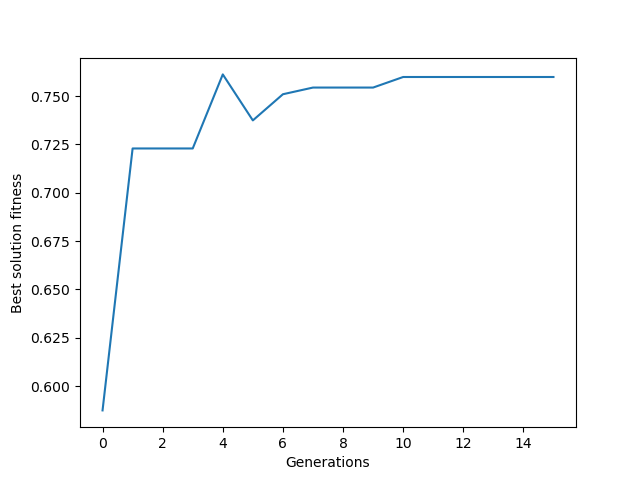
\includegraphics[width=\textwidth]{images/1s.png}
                         \caption*{Περίπτωση: 20, 0.6 ,0.00}
                     \end{subfigure}
                     \hfill
                     \begin{subfigure}[h]{0.7\textwidth}
                         \centering
                         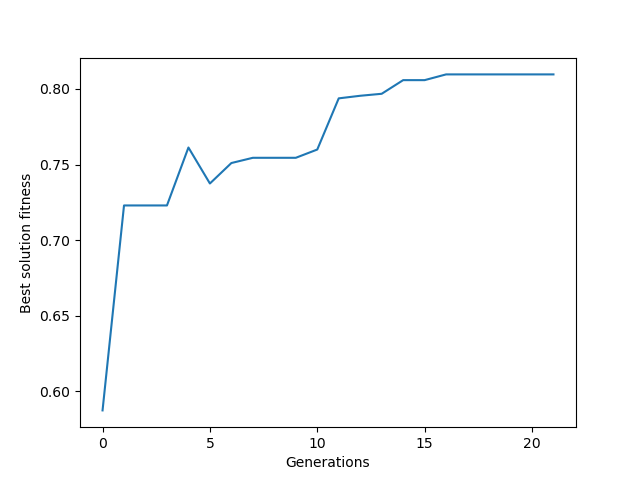
\includegraphics[width=\textwidth]{images/2s.png}
                         \caption*{Περίπτωση: 20, 0.6 ,0.01}
                     \end{subfigure}
                     \hfill
                     \begin{subfigure}[h]{0.7\textwidth}
                         \centering
                         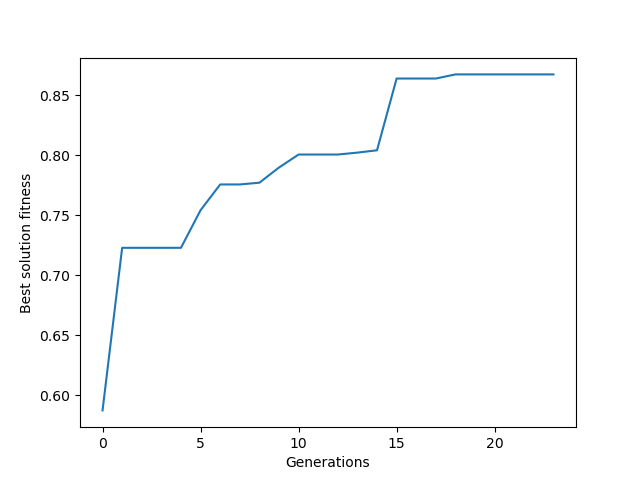
\includegraphics[width=\textwidth]{images/3s.png}
                         \caption*{Περίπτωση: 20, 0.6 ,0.10}
                     \end{subfigure}
                 \end{figure}
                 \begin{figure}[H]
                     \centering
                     \begin{subfigure}[h]{0.7\textwidth}
                         \centering
                         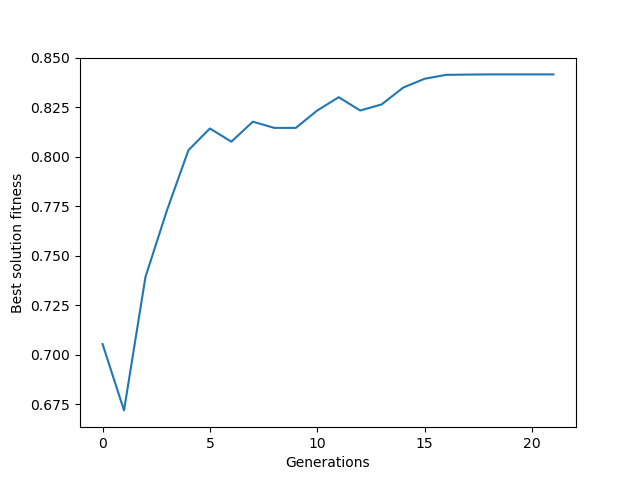
\includegraphics[width=\textwidth]{images/4s.png}
                         \caption*{Περίπτωση: 20, 0.9 ,0.01}
                     \end{subfigure}
                     \begin{subfigure}[h]{0.7\textwidth}
                         \centering
                         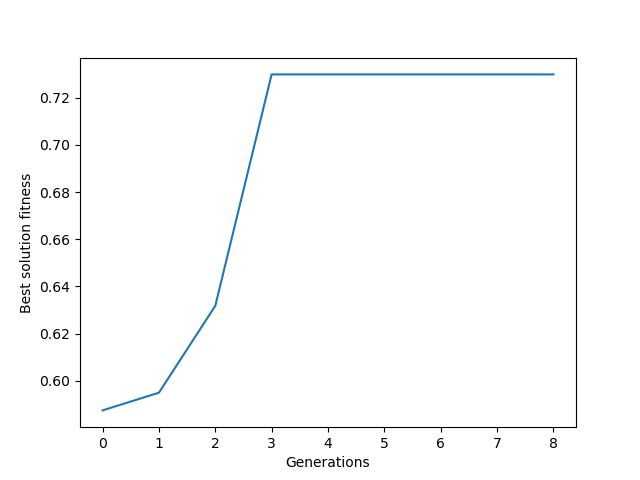
\includegraphics[width=\textwidth]{images/5s.png}
                         \caption*{Περίπτωση: 20, 0.1 ,0.01}
                     \end{subfigure}
                     \begin{subfigure}[H]{0.7\textwidth}
                         \centering
                         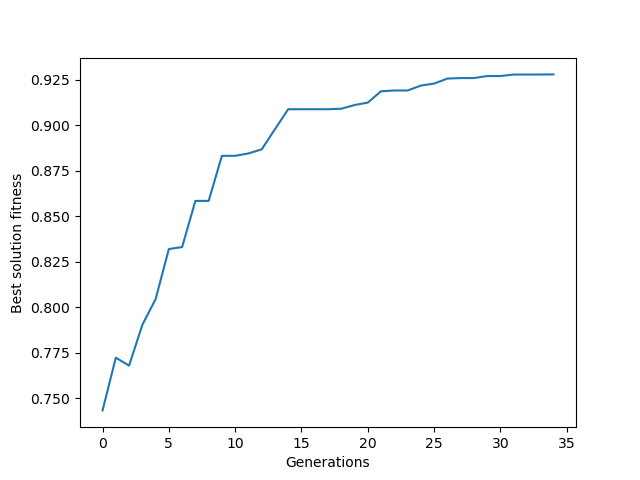
\includegraphics[width=\textwidth]{images/6s.png}
                         \caption*{Περίπτωση: 200, 0.6 ,0.00}
                     \end{subfigure}
                 \end{figure}
                 \begin{figure}[H]
                     \centering
                     \begin{subfigure}[h]{0.7\textwidth}
                         \centering
                         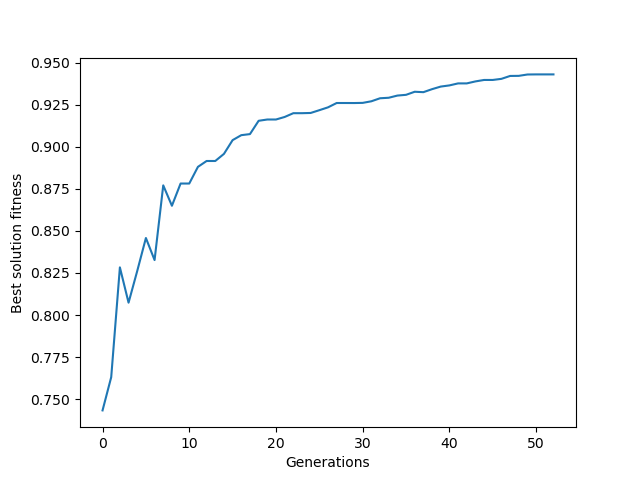
\includegraphics[width=\textwidth]{images/7s.png}
                         \caption*{Περίπτωση: 200, 0.6 ,0.01}
                     \end{subfigure}
                     \begin{subfigure}[h]{0.7\textwidth}
                         \centering
                         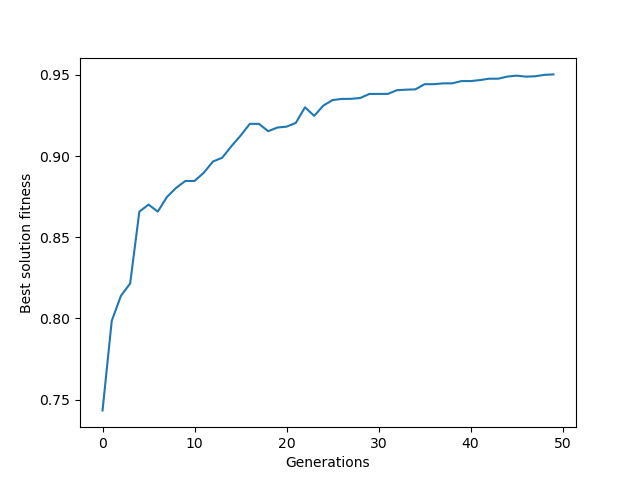
\includegraphics[width=\textwidth]{images/8s.png}
                         \caption*{Περίπτωση: 200, 0.6 ,0.10}
                     \end{subfigure}
                     \begin{subfigure}[h]{0.7\textwidth}
                         \centering
                         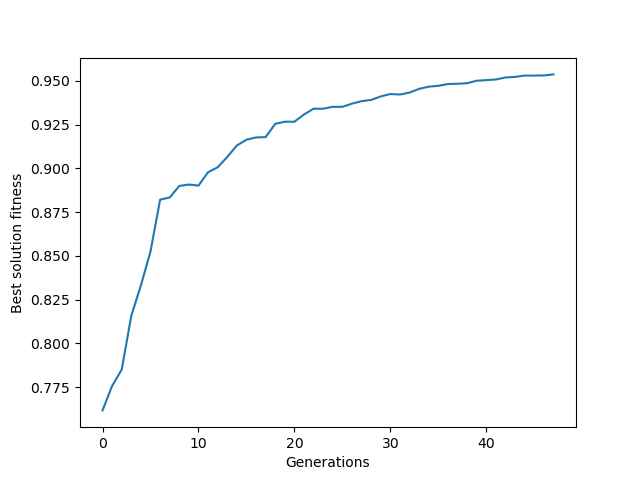
\includegraphics[width=\textwidth]{images/9s.png}
                         \caption*{Περίπτωση: 200, 0.9 ,0.01}
                     \end{subfigure}
                 \end{figure}
                 \begin{figure}[H]
                     \centering
                     \begin{subfigure}[ht]{0.7\textwidth}
                         \centering
                         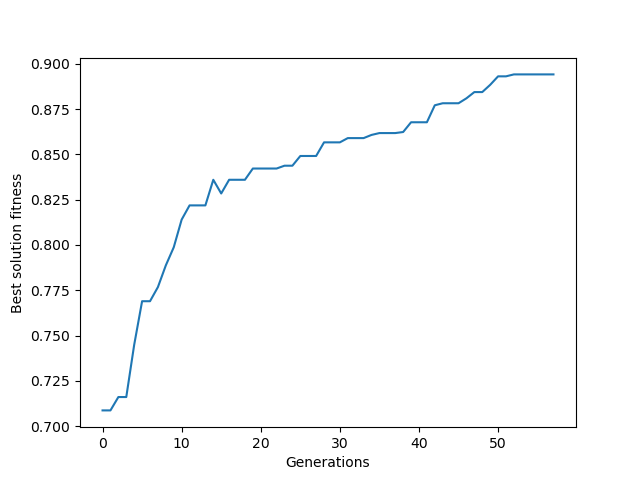
\includegraphics[width=\textwidth]{images/10s.png}
                         \caption*{Περίπτωση: 200, 0.1 ,0.01}
                     \end{subfigure}
                \end{figure} 
            \item Συμπεράσματα: 
                    Σύμφωνα με τα αποτελέσματα που 
                    φαίνονται στον πίνακα και τις γραφικές παραστάσεις, παρατηρούμε αρχικά
                    στις περιπτώσεις που ο αρχικός πληθυσμός
                    είναι 20 έχουμε  μικρή καταλληλότητα για την καλύτερη λύση
                    σε σχέση με πληθυσμό 200 αλλά και
                    ότι η εξέλιξη σταμάτησε σε μικρό αριθμό
                    γενεών πράγμα που σημαίνει ότι η καλύτερη λύση σταμάτησε να βελτιώνεται.
                    Το παραπάνω είναι λογικά αφού λόγω του μειωμένου
                    πληθυσμού έχουμε λιγότερες πιθανότητες να γίνει η διασταύρωση
                    οπότε δεν θα εξεταστεί μεγάλο πλήθος λύσεων. Σε περίπτωση 
                    που δεν είχαμε τα κριτήρια σταματήμου για
                    την εξέλιξη με πληθυσμό 20 ίσως βρίσκαμε κάποια καλύτερη καταλληλότητα
                    μετά από έναν μεγάλο αριθμό γενεών αλλά υπάρχει μεγάλη
                    πιθανότητα αυτή η λύση να μην είναι η βέλτιστη αλλά κάποιο
                    τοπικό βέλτιστο, πράγμα που επιβεβαιώνεται στα διαγράμματα
                    αφού μετά από ένα πλήθος γενεών οι αλλάγες της
                    καταλληλότητας είναι πολύ μικρες. Στο
                    πληθυσμό 200 βλέπουμε ότι τα αποτελέσματα είναι καλύτερα διότι υπάρχει 
                    μεγαλύτερη ποικιλομορφία στα άτομα και περισσότερες
                    πιθανότητες διασταύρωσης, οπότε η
                    εξέλιξη συνεχίζει για αρκετές γενεές. Παρά όμως το γεγονός
                    ότι η καλύτερη λύση έχει πολύ υψηλή καταλληλότητα, ο χρόνος
                    εκτέλεσης ήταν αρκετά υψηλός.\\
                    Στο πίνακα παρατηρούμε ότι η πιθανότητα
                    διασταύρωσης όσο μεγαλύτερη είναι τόσο καλύτερη είναι η τιμή του
                    \tl{fitness} της καλύτερης λύσης αλλά και
                    η εξέλιξη ολοκληρώνεται γρηγορότερα. Άρα, εξαιτίας της μεγαλύτερης
                    πιθανότητας διασταύρωσης τα άτομα 
                    διασταυρώνονται πιο συχνά οπότε η απόγονοι είναι
                    διαφορετκοί από τους γονείς που ισοδυναμεί σε μία
                    καινούργια
                    λύση. Όταν η πιθανότητα διασταύρωσης είναι μικρή βλέπουμε ότι
                    η καλύτερη λύση έχει πολύ μικρή καταλληλότητα διότι οι
                    απόγονοι μοιάζουν πολύ με τους γονείς τους. Τέλος βλέπουμε ότι στον πίνακα ότι
                    η μέση τιμή του βέλτιστου στης περιπτώσεις που η πιθανότητα
                    μετάλλαξης δεν είναι μηδενική ο μέσος αριθμός
                    γενεών αυξάνεται και στην περίπτωση που η τιμή της είναι 0.1
                    έχουμε την καλύτερη μέση τιμή του βέλτιστου.
                    Αυτό συμβαίνει διότι με την μετάλλαξη δίνεται η δυνατότητα στον
                    πληθυσμό να εξερευνήσει μεγαλύτερο πλήθος
                    λύσεων και αποτρέπει τα χρωμοσώματα να γίνουν ίδια μετά από κάποιες
                    γενιές εξέλιξης και να κολλήσουν σε κάποιο τοπικό ακρότατο.
        \end{enumerate}

        \section*{Β4. Αξιολόγηση ΤΝΔ}

            \begin{enumerate}[a)]
                \item
                    \begin{enumerate}[i.]
                        \item Η καλύτερη λύση του γενετικού αλγορίθμου μας έδωσε
                            \tl{accuracy} στα άγνωστα δεδομένα 0.95 ενώ το
                            μοντέλο από την εργασία Α 0.98. Αυτό σημαίνει ότι η
                            καλύτερη λύση του γενετικού μας αλγορίθμου δεν έχει
                            καλύτερη γενικευτική ικανότητα αν και η απόκλιση
                            είναι πολύ μικρή. Ο λόγος που συμβαίνει αυτό είναι
                            που ο γενετικός μας δεν έχει εκπαιδευτεί για όλο το
                            σύνολο δεδομένων του \tl{train} αλλά σε ένα μέρος
                            αυτού(10.000). Η περίπτωση που θα έχει εκπαιδευτεί
                            σε όλο θα εξεταστεί αργότερα.
                            \\
                        \item Παρακάτω παρουσιάζονται δύο εικόνες πριν και μετά
                            την εφαρμογή της επιλογής χαρακτηριστικών σύμφωνα με
                            την καλύτερη λύση: 
                            \begin{figure}[H]
                                \begin{subfigure}{0.5\textwidth}
                                    \raggedleft
                                    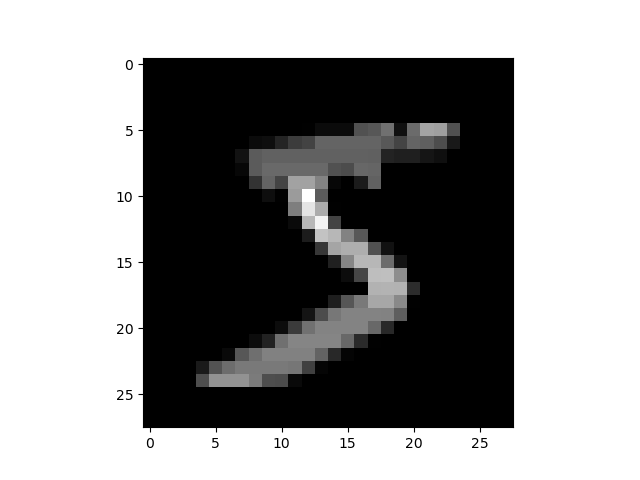
\includegraphics[width=\textwidth]{images/im2.png}
                                \end{subfigure}
                                \begin{subfigure}{0.5\textwidth}
                                    \raggedleft
                                    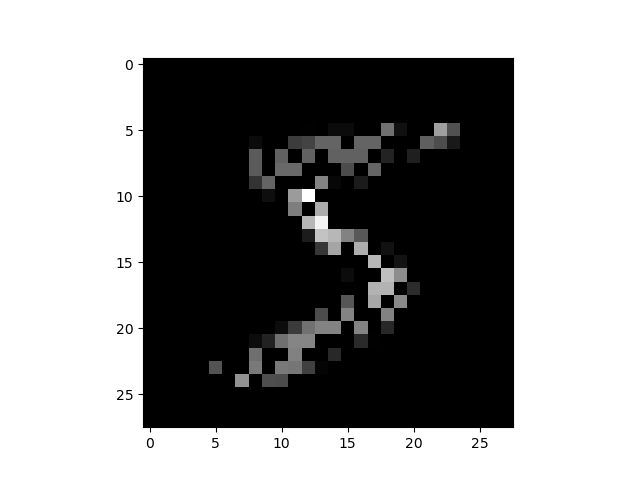
\includegraphics[width=\textwidth]{images/im0.png}
                                \end{subfigure}
                            \end{figure}
                            \begin{figure}[H]
                                \begin{subfigure}{0.5\textwidth}
                                    \raggedleft
                                    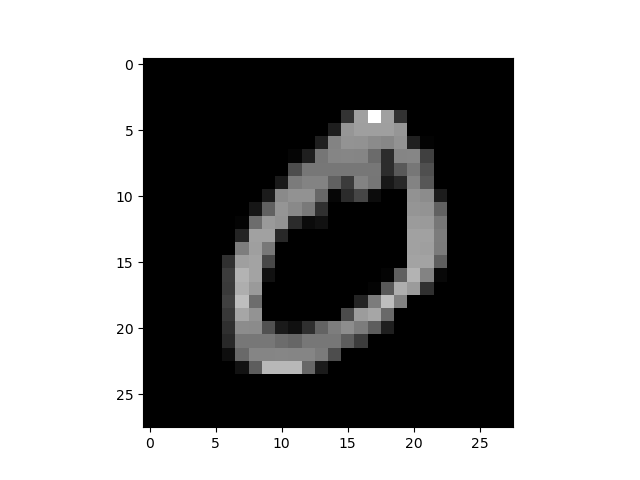
\includegraphics[width=\textwidth]{images/im3.png}
                                \end{subfigure}
                                \begin{subfigure}{0.5\textwidth}
                                    \raggedleft
                                    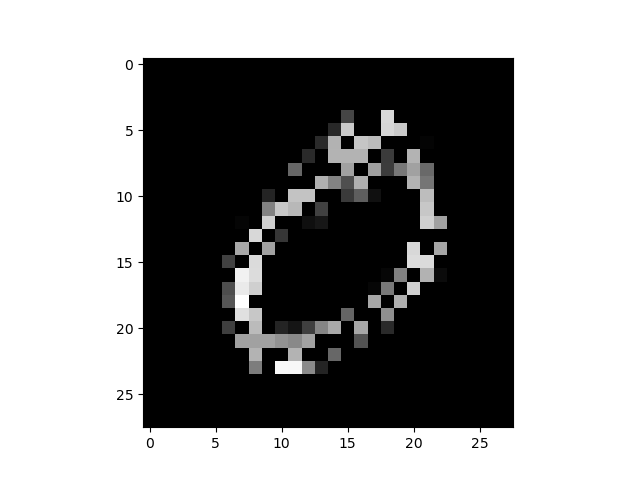
\includegraphics[width=\textwidth]{images/im4.png}
                                \end{subfigure}
                            \end{figure}


                            Παρατηρούμε ότι υπάρχουν κάποιες αφαιρέσεις
                            εικονοστοιχείων από το περίγραμμα του αριθμού το
                            οποίο είναι αναμενόμενο. Υπάρχουν όμως και σημεία
                            πάνω στον αριθμό που έχουν αφαιρεθεί
                            \tl{pixels}, ο λόγος που συμβαίνει αυτό οφείλεται
                            στο γεγονός ότι οι γενετικοί είναι καθαρά
                            μια στοχαστική διαδικασία οπότε δεν μπορούμε να
                            διασφαλίσουμε τη  βέλτιστη λύση το μόνο που μπορούμε
                            είναι να βρούμε κάποια πολύ κοντά σε αυτή.
                        \item Το γεγονός που έχουν αφαιρεθεί εικονοστοιχεία πάνω
                            στον αριθμό δείχνει 
                             κάποια υπερπροσαρμογή στα
                            δεδομένα που εκπαιδεύτηκε ο γενετικός μας
                            αλγόριθμος. Διότι μπορεί να υπήρχαν εικόνες που στα
                            σημεία αυτά να μην περιείχαν τίποτα ή η
                            είσοδος που είχαν να μην επηρέαζε το τελικό
                            αποτέλεσμα οπότε αφαιρέθηκε. Τα σημεία αυτά όμως
                            μπορεί να περιέχουν σημαντική πληροφορία για τις
                            υπόλοιπες εικόνες.

                    \end{enumerate}
                \item

                            \begin{enumerate}[i.]
                                \item Μετά την εξέλιξη του αλγορίθμου σε όλο το
                                    σύνολο τον δεδομένων και τον έλεγχο στο
                                    άγνωστο σύνολο(\tl{mnist\_test}) τα
                                    αποτελέσματα ήταν ίδια με το προηγούμενο σε
                                    ότι αφορά την γενικευτική ικανότητα του
                                    δικτύου.
                                \item Παρακάτω παρουσιάζονται οι ίδιες εικόνες πριν και μετά
                                    την εφαρμογή της επιλογής χαρακτηριστικών: 
                            \begin{figure}[H]
                                \begin{subfigure}{0.5\textwidth}
                                    \raggedleft
                                    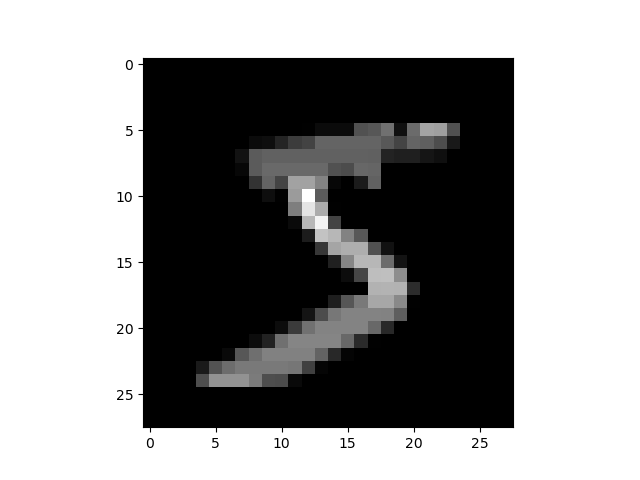
\includegraphics[width=\textwidth]{images/im7.png}
                                \end{subfigure}
                                \begin{subfigure}{0.5\textwidth}
                                    \raggedleft
                                    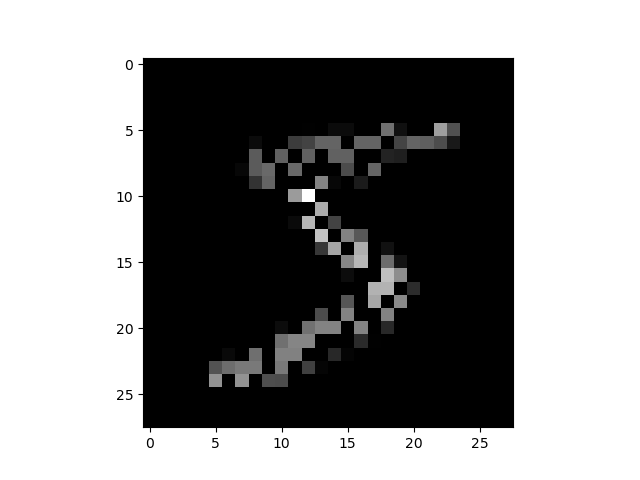
\includegraphics[width=\textwidth]{images/im8.png}
                                \end{subfigure}
                            \end{figure}
                            \begin{figure}[H]
                                \begin{subfigure}{0.5\textwidth}
                                    \raggedleft
                                    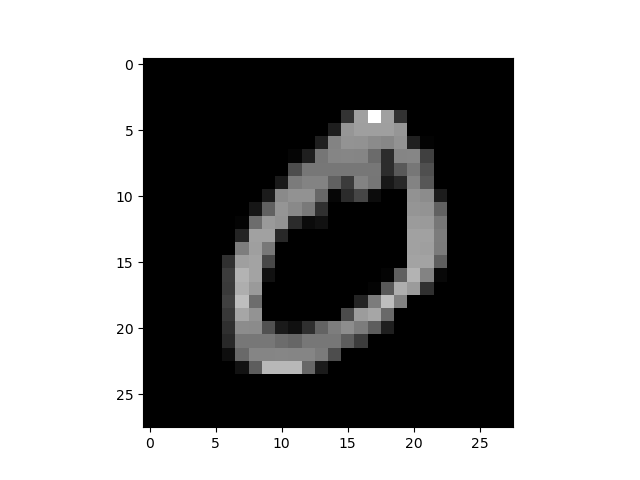
\includegraphics[width=\textwidth]{images/im5.png}
                                \end{subfigure}
                                \begin{subfigure}{0.5\textwidth}
                                    \raggedleft
                                    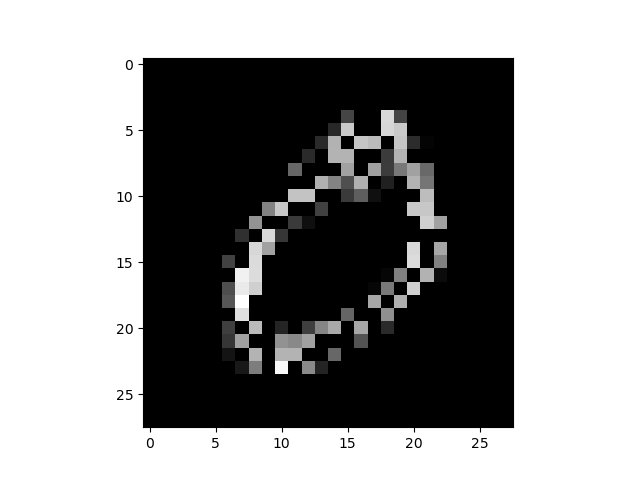
\includegraphics[width=\textwidth]{images/im6.png}
                                \end{subfigure}
                            \end{figure} 
                                παρατηρείται ότι οι εικόνες και στις δύο
                                    διαφορετικές περιπτώσεις είναι σχεδόν ίδιες, Αυτό μας οδηγεί στο
                                    συμπέρασμα ότι η βέλτιστη λύση και στις δύο
                                    περιπτώσεις είναι ίδια ανεξαρτήτως του
                                    αριθμού των εικόνων. Οι μικρές διαφορές που
                                    υπάρχουν οφείλεται στη στοχαστική φύση του
                                    αλγορίθμου αλλά σύμφωνα με το γεγονός ότι
                                    δεν αλλάζει η ακρίβεια του νευρωνικού
                                    σημαίνει ότι οι διαφορές που υπρχουν δεν
                                    ήταν σε \tl{pixels} που παρείχαν πολύτιμη
                                    πληροφορία.
        
                                \item Εφόσον εξεταστικές και αυτή η περίπτωση
                                    και τα αποτελέσματα είναι ίδια, η
                                    υπερπροσαρμογή είναι αρκετά απίθανη και αυτό
                                    είναι λογικό αν αναλογιστούμε τα δεδομένα
                                    που έχουμε. Το \tl{dataset} είναι αρκετά
                                    \tl{optimized} για τέτοιου είδους
                                    προβλήματα. Ουσιαστικά οι εικόνες
                                    κατανέμονται ομοιόμορφα μέσα στο
                                    \tl{dataset} αρά στην πρώτη περίπτωση που ο
                                    αλγόριθμος έτρεξε για μικρότερο πλήθος
                                    δεδομένων αρκούσε ώστε να δει αρκετές
                                    εικόνες και να καταλήξει σε αυτή τη λύση.

        
                            \end{enumerate}
            \end{enumerate}
\end{document}
